\documentclass{article}
\usepackage{geometry}
\usepackage{paralist}
\usepackage[T1]{fontenc}
\usepackage{reledmac}
\usepackage{changepage}
\usepackage{amsmath}
\usepackage{scalerel,amssymb}

\usepackage{graphicx}
\graphicspath{{./Images/}}

\usepackage{pgfplots}
\usepackage{tikz}
\usetikzlibrary{positioning}
\usetikzlibrary{shapes.geometric, arrows}
\tikzstyle{arrow} = [thick,->,>=stealth]

\usepackage{fancyhdr}
\fancyhead[L]{
	\begin{tabular}{l}
		\LARGE \textbf{\textsc{Concurrency}} \\
		\Large Assignement 04
	\end{tabular}
}
\fancyhead[R]{
	\begin{tabular}{r}
		16-124-836 \\
		Marcel \textsc{Zauder}
	\end{tabular}
}
\renewcommand{\headrulewidth}{0.4pt}
\fancyfoot[C]{\thepage}
\renewcommand{\footrulewidth}{0.4pt}

\usepackage{hyperref}

\begin{document}
	\pagestyle{fancy}
	\section{Smoothing with Heartbeat}
	\begin{adjustwidth}{2em}{2em}
		\subsection{Implementation}
		\begin{adjustwidth}{2em}{2em}
			The images can be found in the $src/Executors/Images$ folder. In there the original pgm-files are saved. For each modify-algorithm seperated folders are used so it can be easily differentiate which picture was generated by which implementation. \\
			The split up algorithm divides the number of rows by the number of threads and gives each thread a vertical section of the image. If there are more threads than rows in the picture the redundant threads are not instantiated (for example if a picture only have 5 rows, at max 5 threads can modify this picture). \\
			For both exercises the "Heartbeat" paradigm is used. It is implemented by using a \textbf{Broadcast} system which allows each thread to send and receive information when they have subscribed to this broadcast. The messages are sent to a buffer and can be fetched by every thread if the heartbeat occurs.
		\end{adjustwidth}
		\subsection{Evaluation}
		\begin{adjustwidth}{2em}{2em}
			The greater the value of $D$ gets the darker the image becomes because a pixel needs more alive neighbours to stay alive. \\
			For the scenario if $D$ is equal to 5 the corners are set to black, then the edges recursively have only 4 neighbours and are disabled as well. Therefore the image will be eventually fully disabled. The higher $D$ is the faster this process gets. \\
			For $D = 3$ not much will happen because not many pixels have only 2 or less alive neighbours. Therefore the pictures look pretty much the same when running this scenario.
			\subsubsection{Influence of Number of Threads}
			\begin{adjustwidth}{1em}{}
				When modifying all pictures one thread needs for $D = 5$ in total $\approx 125$ seconds. With 4 threads the same procedure needs 56 seconds, whereas with 8 threads the algorithm needs 112 seconds. \\
				For $D = 7$ the same behaviour can be observed. 1 Thread needs 42 seconds, 4 threads 21 seconds and 8 threads need 38 seconds. \\
				It can be concluded that the broadcast generates a huge overhead and the synchronization of each thread, while waiting for the next heartbeat takes a lot of time. Therefore the speedup is negligible for 8 threads and not very high for 4 threads as well (with only factor $\approx 2$).
			\end{adjustwidth}
		\end{adjustwidth}
    \end{adjustwidth}
    
    \section{Filter}
    \begin{adjustwidth}{2em}{2em}
    	\subsection{Implementation and General Information}
    	\begin{center}
    		\begin{tabular}{lll}
    			\begin{tabular}{c}
    				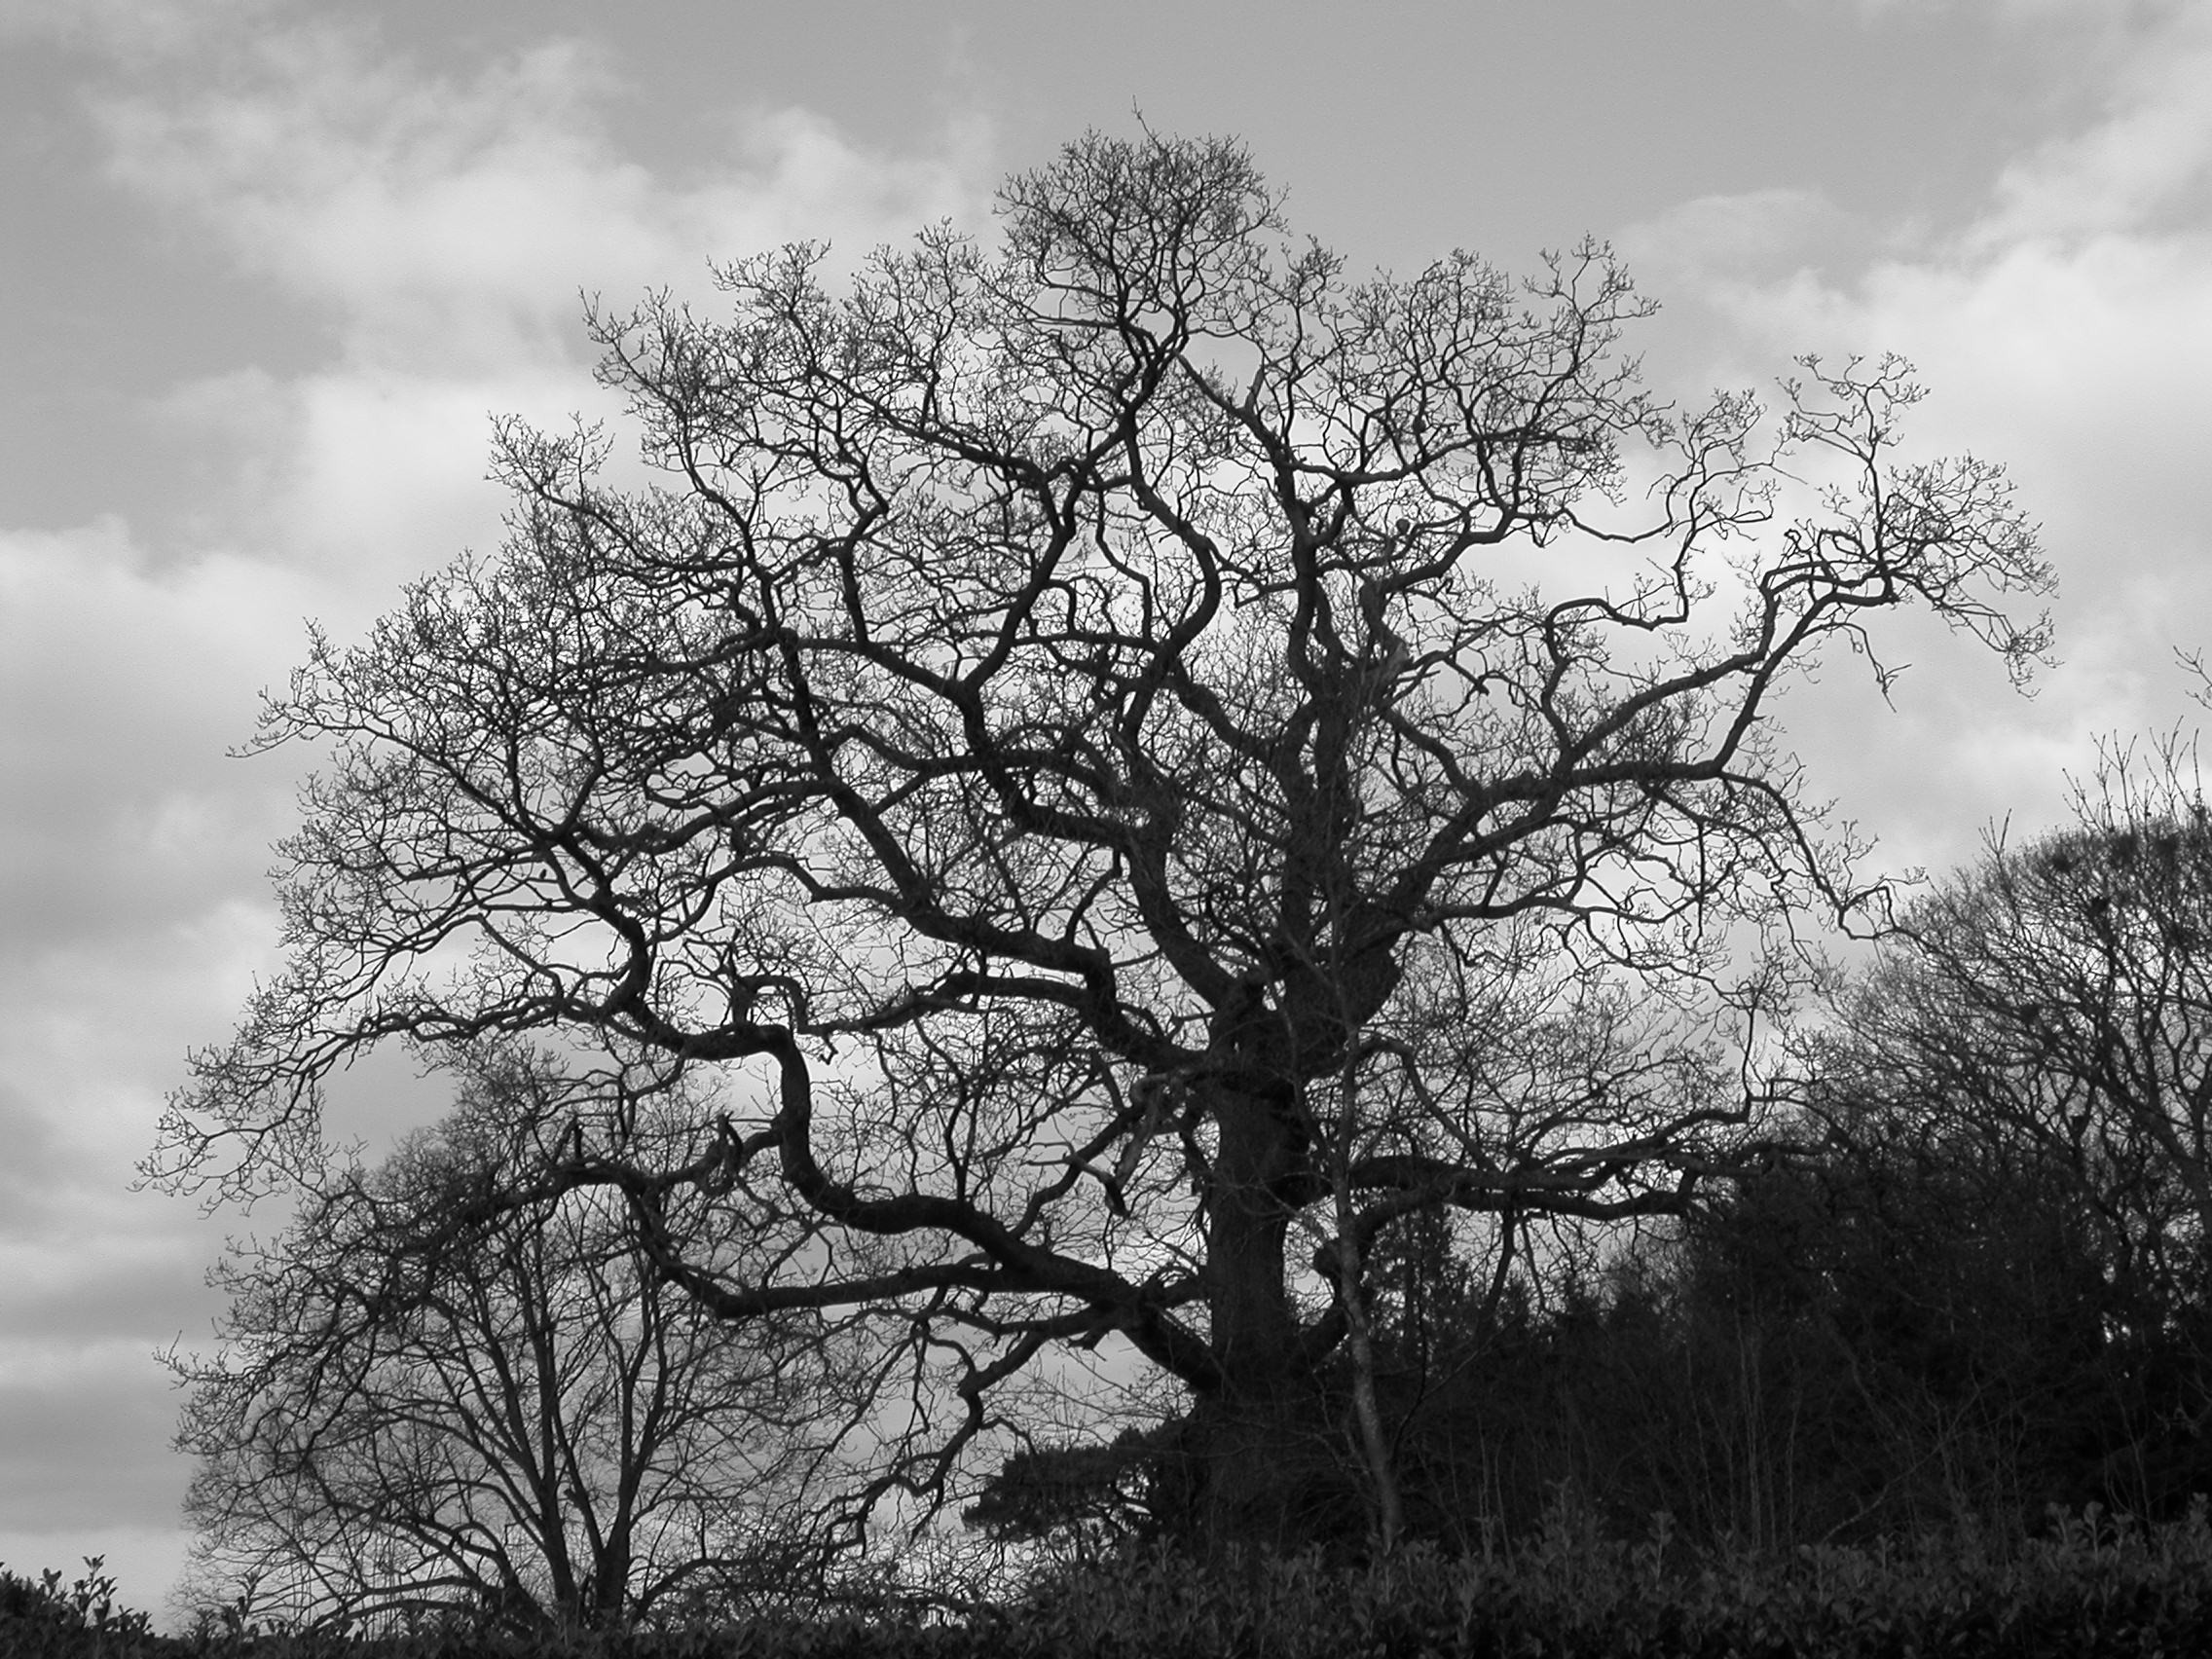
\includegraphics[scale=0.05]{fractal_tree.png}
    			\end{tabular}
    			&
    			&
    			\begin{tabular}{p{5cm}}
    				One of the original pictures with which the implementation was tested.
    			\end{tabular}
    		\end{tabular}
    	\end{center}
    	\begin{adjustwidth}{2em}{2em}
			We tried to implement all different filters. For the "Blur" and "Emboss"-Filter the implementation works pretty much as expected. For the other filters the output is not what was expected by applying the filter. \\
			Every filter algorithm implements a scale factor because by applying the matrix computation it is likely that a value exceed the value of 255 which would lead to a totally white picture.
		\end{adjustwidth}
    	\subsection{Blur-Filter}
		\begin{center}
    		\begin{tabular}{lll}
    			\begin{tabular}{c}
    				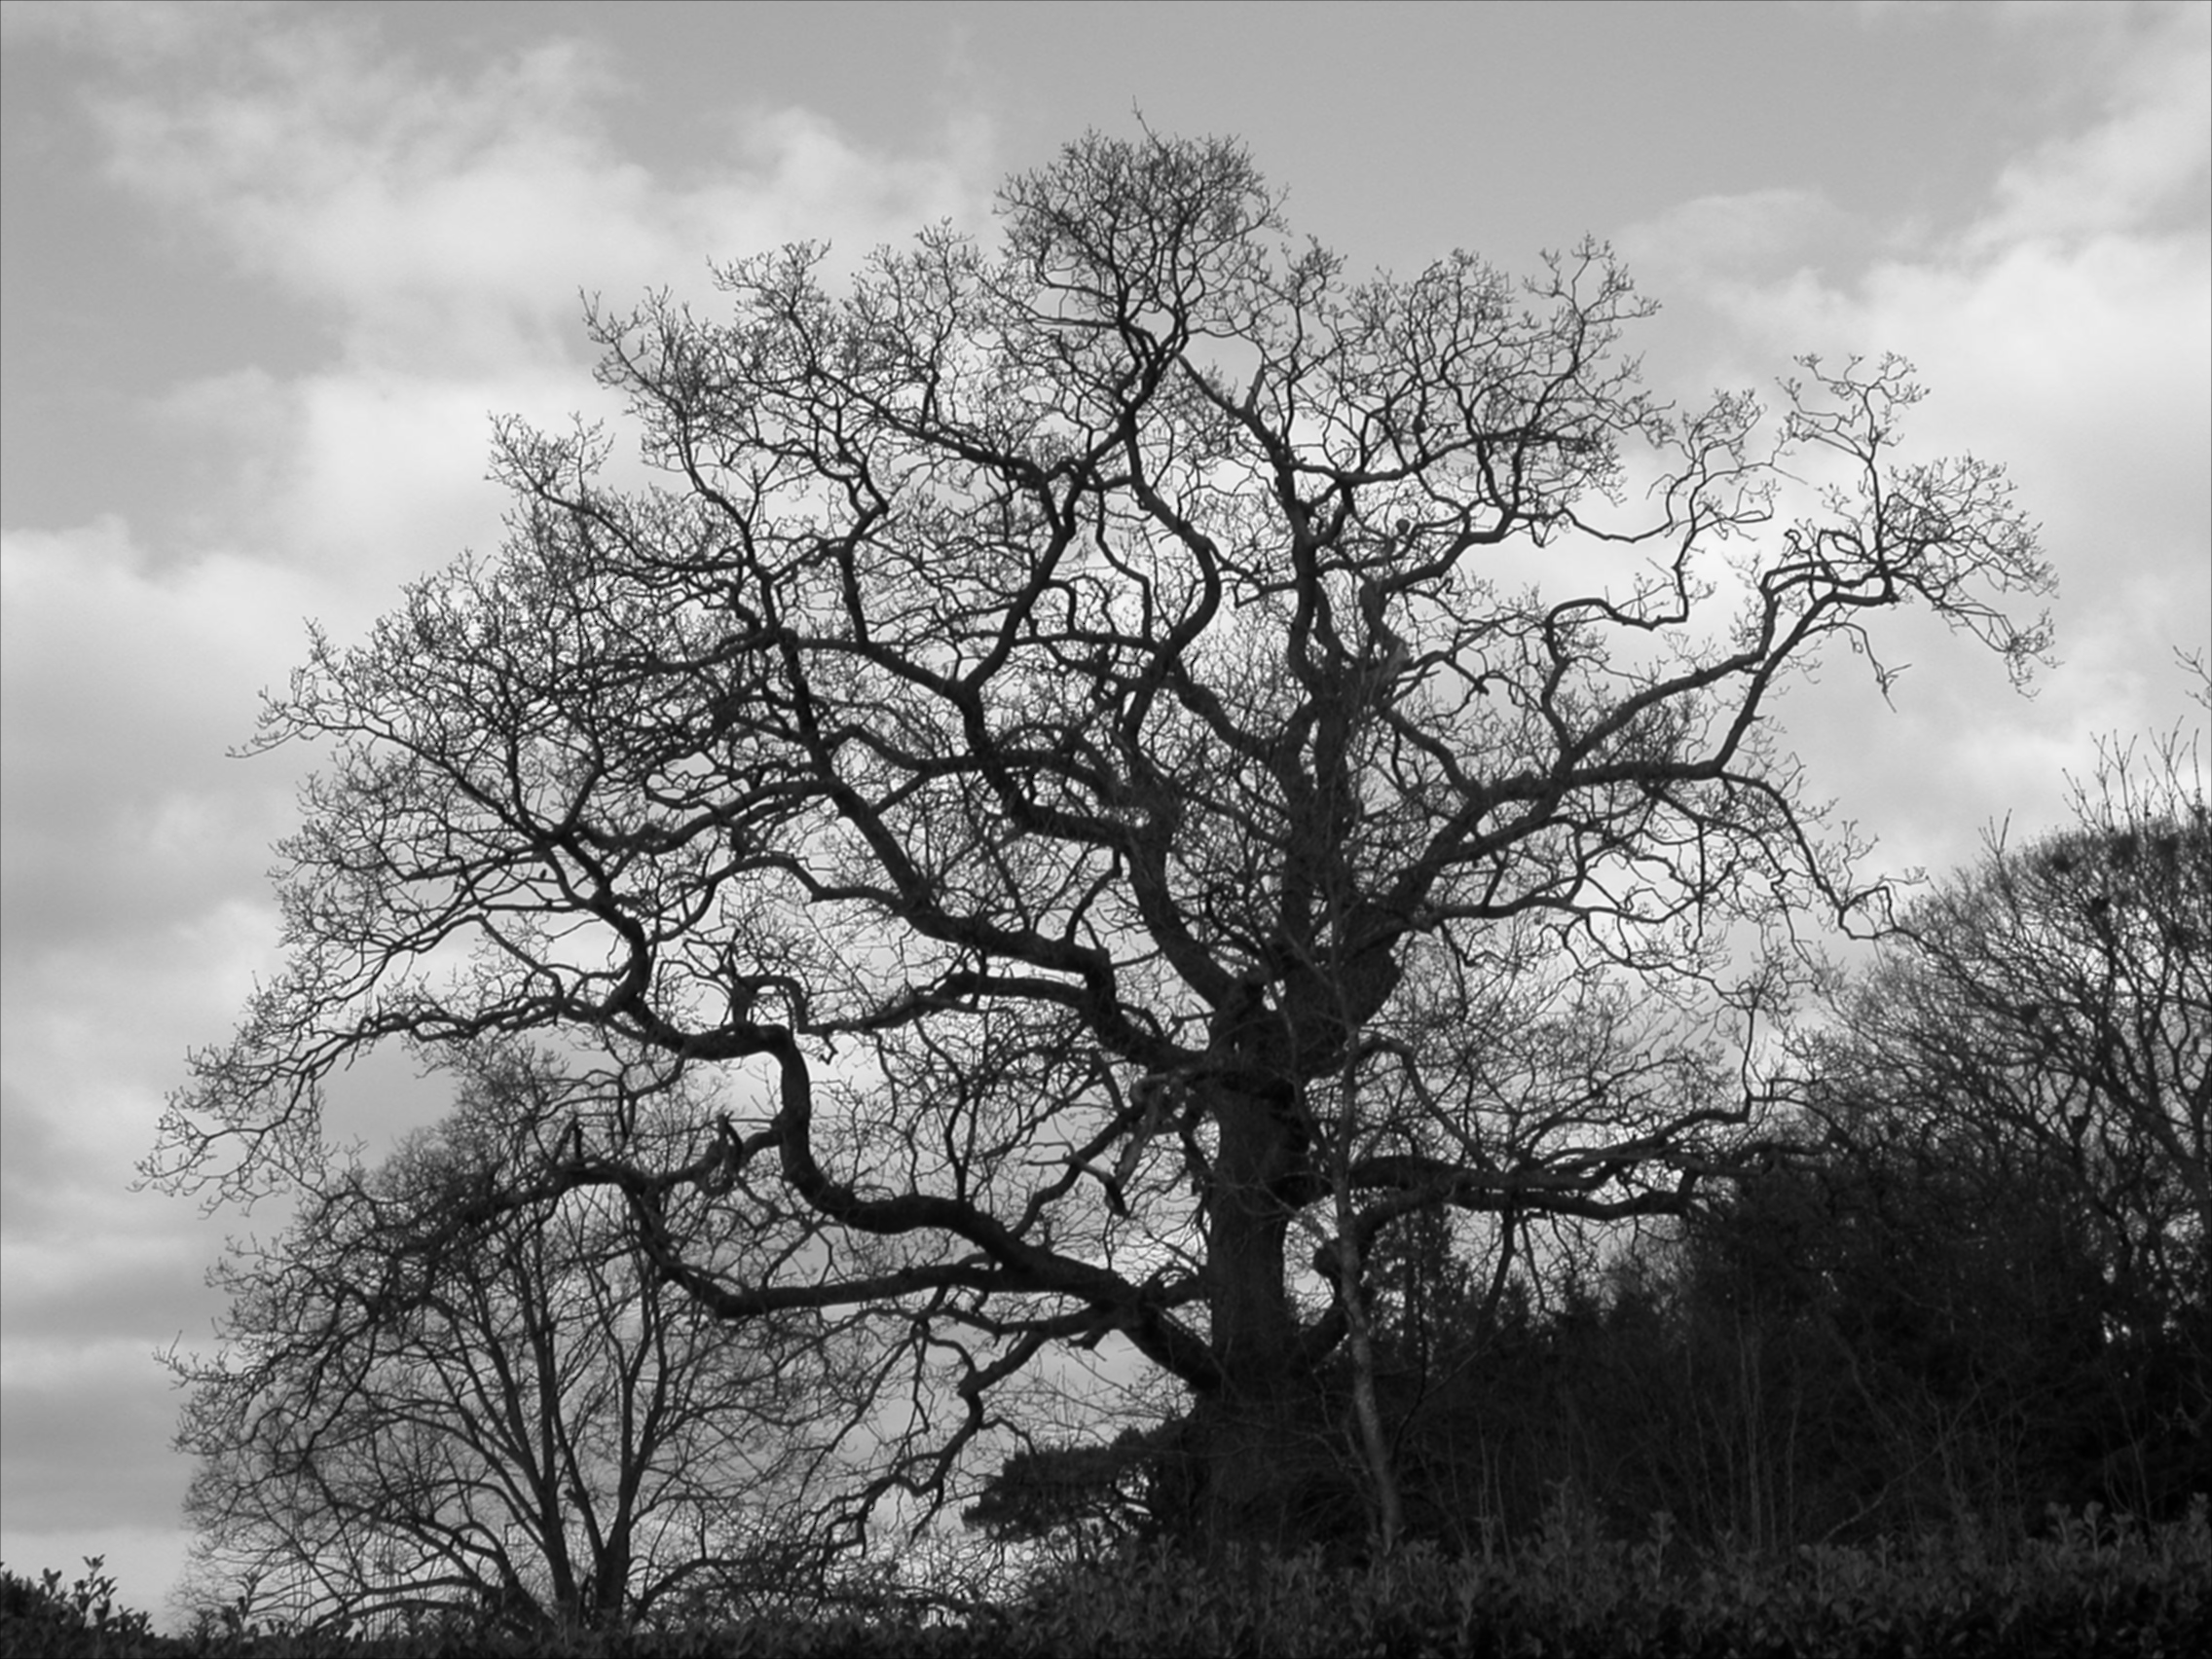
\includegraphics[scale=0.05]{fractal_tree_blur.png}
    			\end{tabular}
    			&
    			&
    			\begin{tabular}{p{5cm}}
    				The blurring effect works as expected.
    			\end{tabular}
    		\end{tabular}
    	\end{center}
		\subsection{Emboss-Filter}
		\begin{center}
    		\begin{tabular}{lll}
    			\begin{tabular}{c}
    				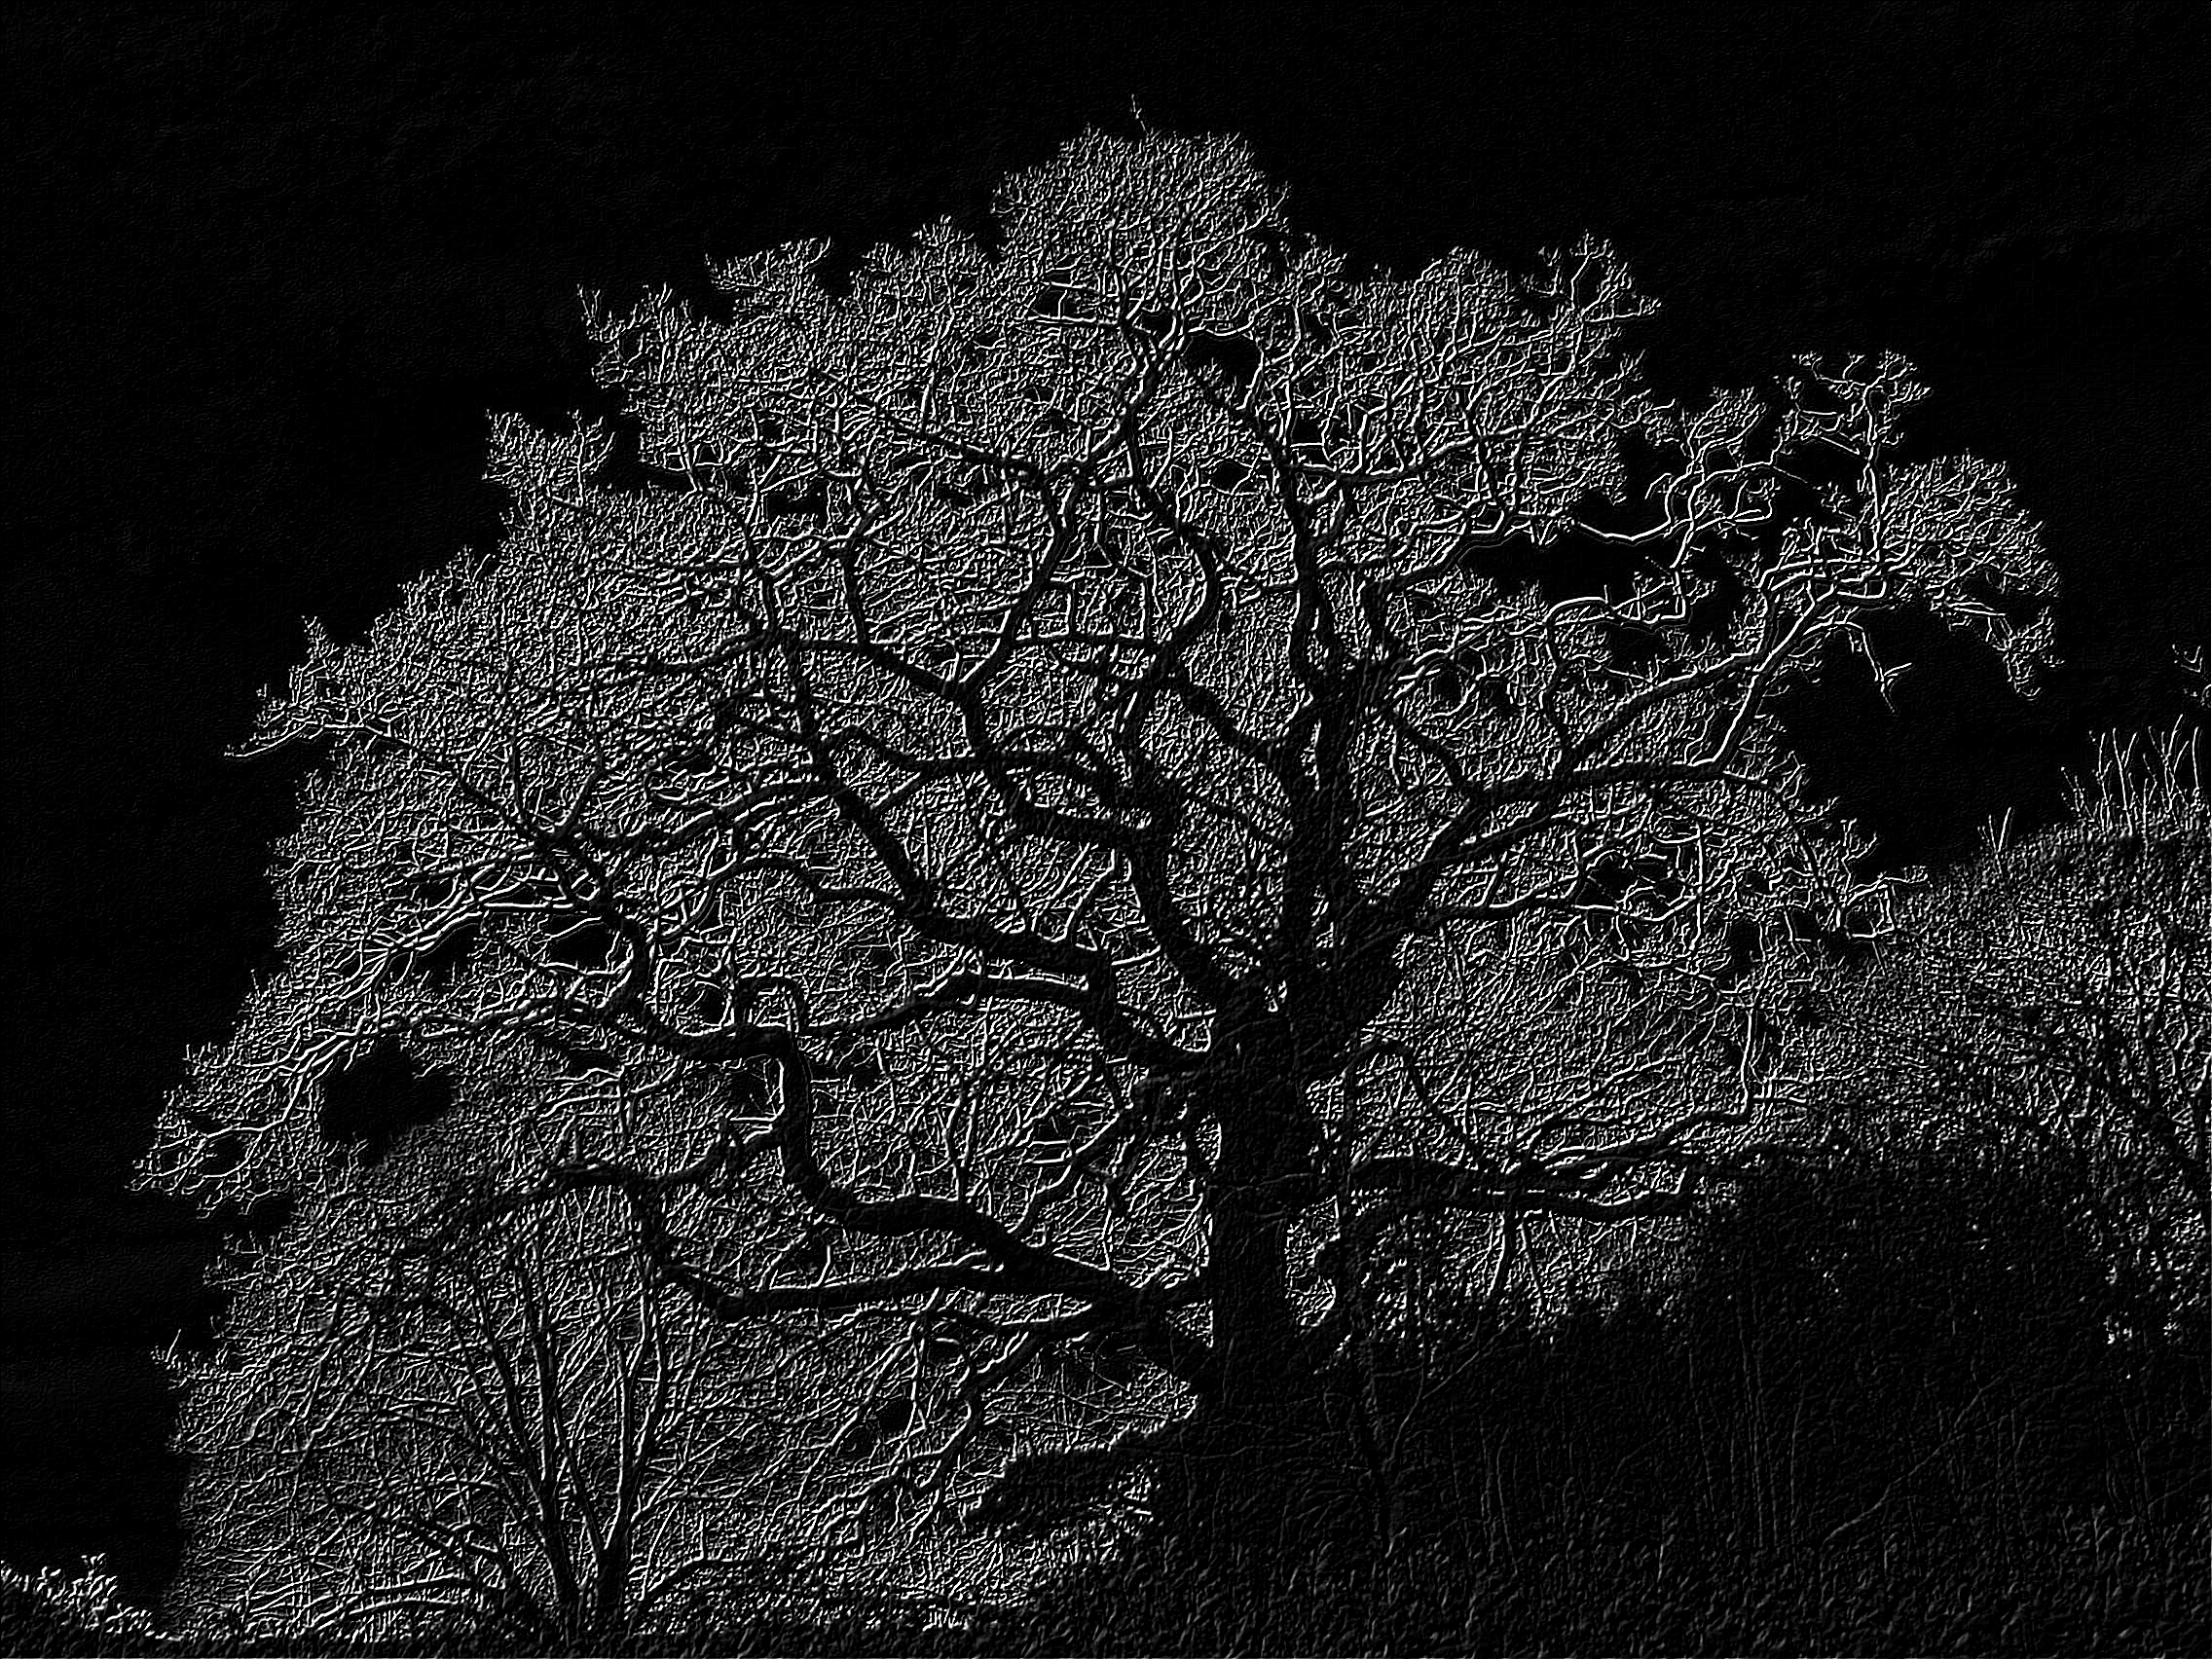
\includegraphics[scale=0.05]{fractal_tree_emboss.png}
    			\end{tabular}
    			&
    			&
    			\begin{tabular}{p{5cm}}
    				The emboss filter produces a picture where only the edges are highlighted and the rest is black (normally it should be more like a grayscale around the edges).
    			\end{tabular}
    		\end{tabular}
    	\end{center}
    	\subsection{Implementation and General Information}
    	\begin{adjustwidth}{2em}{2em}
			The speedup for these algorithms is negligible because the preparation of the picture (reading the image, splitting it and so on) takes most of the time and the actual manipulation only takes a single iteration. Therefore the speedup is nearly 1.
		\end{adjustwidth}
    \end{adjustwidth}    

\end{document}